\begin{enumerate}[label=\alph*)]
  \item On définit la matrice $A$ et le vecteur $\BoldB$ avec les commandes suggérées dans l'énoncé :
  
\begin{verbatim}
  f = @(x) x.*(1-x);
  N = 20; h = 1/N;
  x = linspace(h, 1-h, N-1)'; 
  b = f(x);
  A = (N^2)*(diag(2*ones(N-1, 1),0) - diag(ones(N-2,1),1) - diag(ones(N-2,1),-1));
\end{verbatim}
        
        Ensuite, on calcule la factorisation $LU$ de $A$.
        En général, \textsc{MATLAB} peut décider d'effectuer des permutations de lignes pendant le processus de factorisation, ce qui mène à une factorisation $PA = LU$.
        Ainsi, la syntaxe de la commande \texttt{lu} à utiliser est la suivante :
        
\begin{verbatim}
  [L,U,P] = lu(A);
\end{verbatim}
        
        De cette façon, on a stocké dans la variable \texttt{P} la matrice de permutation $P$.
        Dans notre cas, on peut vérifier que \texttt{P} est la matrice identité : par exemple, on peut calculer l'écart maximal entre les éléments de $P$ et de $I$, et on obtient :
  
\begin{verbatim}
  max(max(abs(P - eye(N-1))))
  ans =
      0
\end{verbatim}
        
        Donc, \textsc{MATLAB} calcule la factorisation $LU$ sans permutation.
        Les facteurs ont été stockés dans les variables \texttt{L} et \texttt{U}.
        Ces facteurs diffèrent du facteur $H$ de la factorisation de Cholesky $A = H H^{\top}$, que l'on calcule avec la commande
  
\begin{verbatim}
  H = chol(A)';
\end{verbatim}
        
        car
        
\begin{verbatim}
  max(max(abs(L - H)))
  ans =
      27.2843
\end{verbatim}
        
  \item On trouve
  
        \lstinputlisting{s3/matlab/subs_directe.m}
        \lstinputlisting{s3/matlab/subs_retrograde.m}
        
        D'après le cours, on exploite la factorisation $LU$ de la façon suivante :
        
\begin{verbatim}
y = subs_directe(L,b);
u = subs_retrograde(U,y);
\end{verbatim}
        
  \item La Figure \ref{fig:solExacte} montre les déplacements $u_{i}$ aux noeuds $x_{i}$ (cercles rouges).
        Si $f \parent{x}$ est un polynôme, il est facile de trouver la solution exacte du problème différentiel : dans notre cas \footnote{Comme $u'' \parent{x} = - x + x^{2}$,
        on intègre deux fois et on trouve $u \parent{x} = x^{4} / 12 - x^{3} / 6 + a x + b$, où $a$ et $b$ sont deux constantes que l'on trouve en imposant les conditions aux bords :
          \begin{equation*}
            u \parent{0} = 0 \Longrightarrow b = 0, 
            \quad \quad
            u \parent{1} = 0 \Longrightarrow a = 1/12.
          \end{equation*}},
        on a $u \parent{x} = x^{4} / 12 - x^{3} / 6 + x / 12$.
        On a ajouté le graphe de $u \parent{x}$ afin de montrer qu'avec $N = 20$ sous-intervalles, on obtient déjà une solution approchée assez précise.
        La Figure \ref{fig:solExacte} a été obtenue par le script \texttt{ex2exact.m} suivant.
        
        \lstinputlisting{s3/matlab/ex2exact.m}
        
        
\begin{figure}[h!]
  \centering
  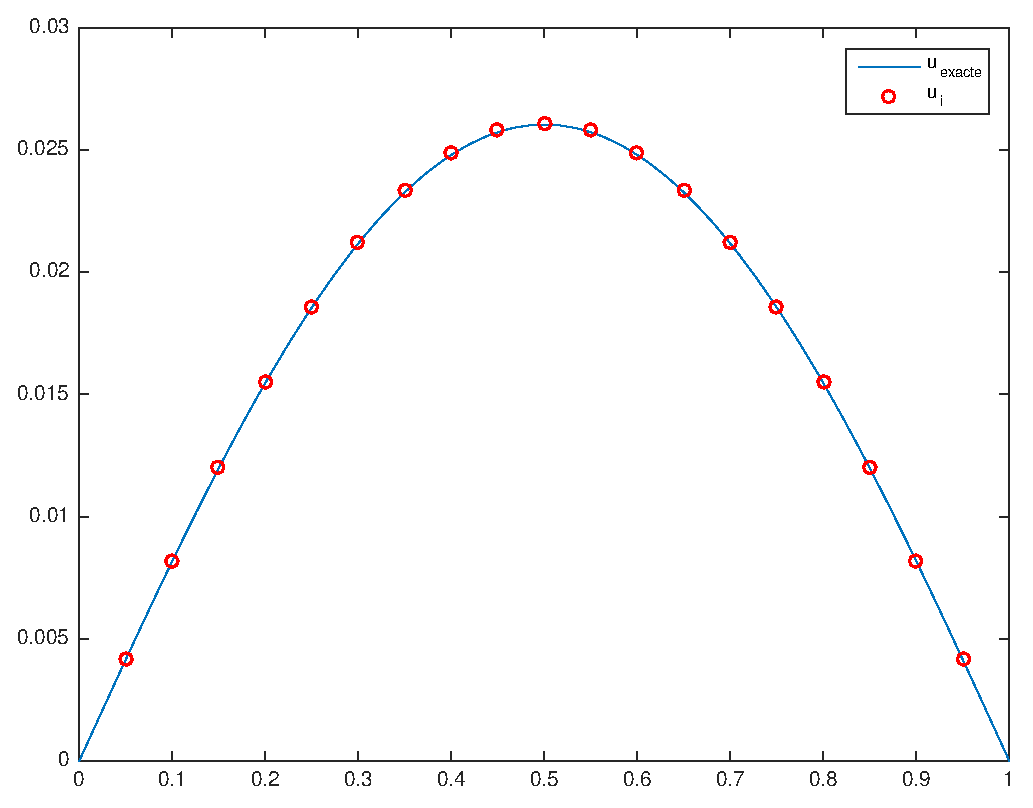
\includegraphics[scale = 0.5]{s3/matlab/ex2_uexact.eps}
  \caption{Solution exacte $u \parent{x}$ et déplacements approchés $u_{i}$}
  \label{fig:solExacte}
\end{figure}

        Il faut remarquer que la taille du vecteur $\BoldU$ est $N - 1$; en effet seules les valeurs des déplacements aux noeuds $x_{i}$ pour $i = 1, \dots, N - 1$ sont inconnues, car $u_{0} = u_{N} = 0$ (conditions aux bords).
        
  
  \item Pour chaque valeur de $N$, on a une matrice $A$ différente.
        Donc, il faut coder une boucle qui, pour $N = 10, 20, 30, \dots, 120$, construit cette matrice et calcule son conditionnement.
        Cette valeur sera ensuite mémorisée dans un vecteur \texttt{k}.
        La boucle peut se coder comme suit : 
        
\begin{verbatim}
for N = 10:10:120
  h = 1/N;
  A=(N^2)*(diag(2*ones(N-1,1),0)-diag(ones(N-2,1),1)-diag(ones(N-2,1),-1));
  k(N/10) = cond(A);
  disp(sprintf('N = %i: K(A) = %e',N,k(N/10)));
  % ceci pour afficher les valeurs calculees
end
\end{verbatim}        
        
        et on obtient
 
\begin{verbatim}
N = 10: K(A) = 3.986346e+01
N = 20: K(A) = 1.614476e+02

(...)

N = 110: K(A) = 4.903279e+03
N = 120: K(A) = 5.835434e+03
\end{verbatim} 

    Le graphe de $K \parent{A}$ en fonction de $N$ (commande \texttt{plot([10:10:120], k))} et le graphe bi-logarithmique (commande \texttt{loglog([10:10:120],k); grid on}) sont affichés en Figure \ref{fig:cond}.
    On peut trouver cette figure avec le script \texttt{ex2bilog.m}.
    
    \lstinputlisting{s3/matlab/ex2bilog.m}
    
    On voit que le graphe bi-logarithmique est bien celui d'une droite, donc du type
    
    \begin{equation*}
      \log_{10} K = m \log_{10} N + c.
    \end{equation*}
    
    On calcule $m$ et $c$ directement sur le graphe, en mesurant la pente entre les abscisses 1 $\parent{N = 10}$ et 2 $\parent{N = 100}$, ou bien en utilisant \MAT :
    
\begin{verbatim}
m = ( log10(k(10)) - log10(k(1)) ) / (log10(120) - log10(10))
m =
    2.0066
    
c = log10(k(1)) - m*log10(10)
c = 
    -0.4060
    
C = 10^c
C =
    0.3926
\end{verbatim} 

\begin{figure}[h!]
  \begin{subfigure}[b]{0.5\linewidth}
    \centering
    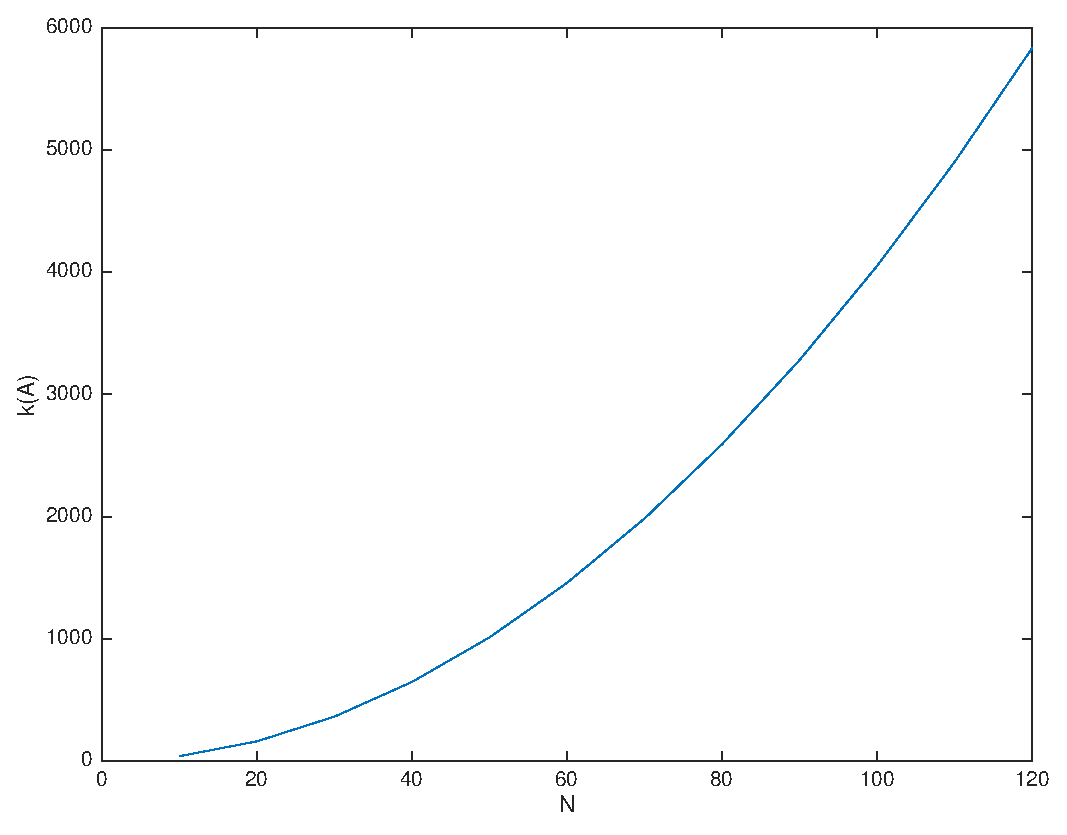
\includegraphics[scale=0.4]{s3/matlab/ex2_lin} 
    %\caption{Interpolation of $f$ using NCS \\ with $8+2$ points} 
    %\label{fig:q11_n8} 
  \end{subfigure}
  \begin{subfigure}[b]{0.5\linewidth}
    \centering
    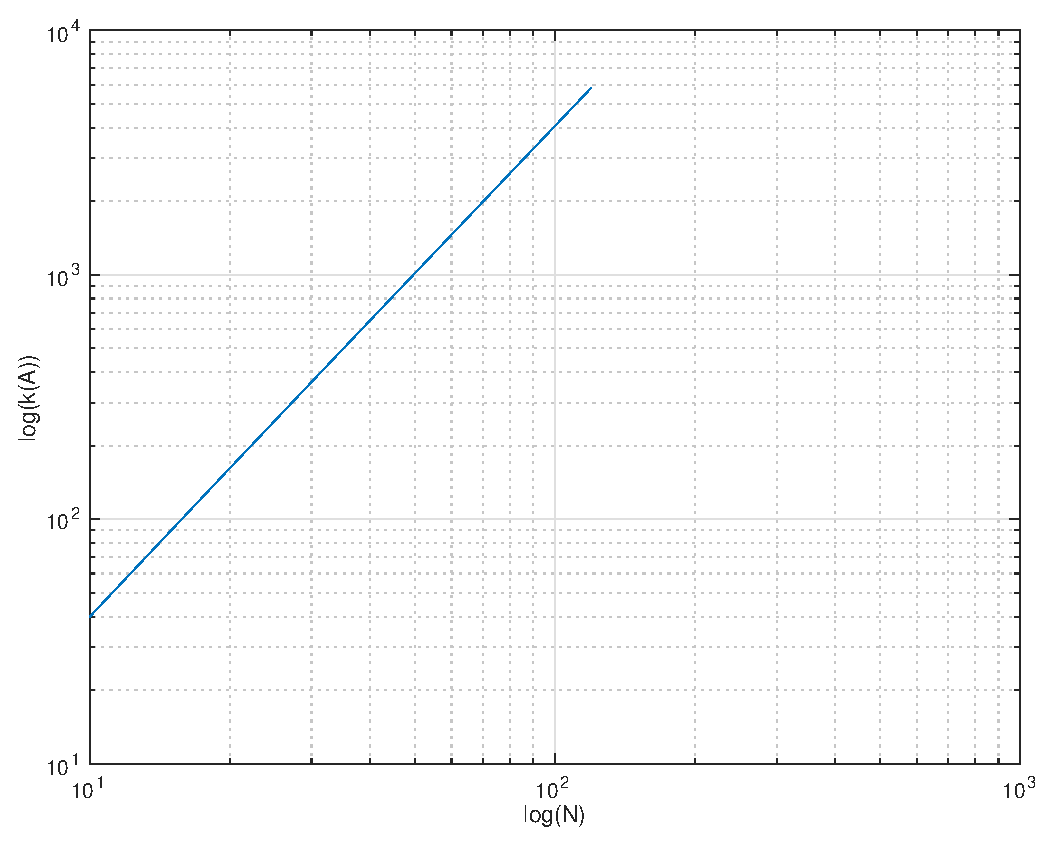
\includegraphics[scale=0.4]{s3/matlab/ex2_log} 
    %\caption{Interpolation of $f$ using NCS \\ with $8+2$ points} 
    %\label{fig:q11_n8} 
  \end{subfigure} 
  \caption{Nombre de conditionnement $K \parent{A}$ en fonction de $N$, graphes linéaire (à gauche) et bi-logarithmique (à droite)}
  \label{fig:cond}
\end{figure}

      La pente est presque égale à 2, donc la formule à proposer sera bien
      
      \begin{equation*}
        K \parent{A} = C N^{2}
      \end{equation*}
      
       avec $C \simeq 0.3926$.
       Donc, $K \parent{A}$ croît quadratiquement avec $N$, ce qui signifie que la solution du système linéaire par la méthode de factorisation $LU$ devient de plus en plus sensible aux perturbations sur les données et aux erreurs d'arrondi.

  


         
         
         
  
  
\end{enumerate}